% =============================================================================
% Paper 2 — Rectangular T^3 Casimir stress and free-field biaxial backreaction
% Genre: technical paper (validated mechanism + negative free-field attractor)
% Class: Physical Review D (revtex4-2)
% Claim firewall: papers/Selective-Publishing-Plan (B1–B16 packaging bans)
% =============================================================================
\documentclass[aps,prd,reprint,superscriptaddress,nofootinbib,floatfix]{revtex4-2}

\usepackage[T1]{fontenc}
\usepackage[utf8]{inputenc}
\usepackage{amsmath,amssymb,amsthm}
\usepackage{booktabs}
\usepackage{graphicx}
\usepackage[hidelinks]{hyperref}

\graphicspath{{figures/}{../../Assets/Figures/}{../../Analysis/Casimir/CBR-001/stage2_outputs/}{../../Analysis/Casimir/CBR-001/stage3b_outputs/}}

\newcommand{\Tthree}{T^{3}}
\newcommand{\Ht}{H_{t}}
\newcommand{\Hp}{H_{p}}

\begin{document}

\title{Anisotropic Casimir stress on rectangular flat
\texorpdfstring{\(\Tthree\)}{T3} and the absence of a free-field
\texorpdfstring{\(\Ht/\Hp=13/12\)}{Ht/Hp=13/12} attractor}

\author{Brendon Boyd}
\email{brendon.boyd@itsm-cosmology.org}
\affiliation{Independent Researcher, Burswood, Western Australia, Australia}
\thanks{ORCID: \href{https://orcid.org/0009-0007-4177-2612}{0009-0007-4177-2612}.
Code and claim ledger:
\url{https://github.com/brendohxd/ITSM-Integrated-Toroidal-Syntropic-Model};
reproducible gate package: \texttt{Analysis/Casimir/CBR-001/}.}

\date{\today}

\begin{abstract}
Compact spatial topology can source anisotropic vacuum stress.
For a free massless scalar on a rectangular flat three-torus we validate a
renormalized lattice Casimir energy density and directional pressures
(cutoff convergence, cubic isotropy, thermodynamic pressure derivatives,
conformal trace, and dimensional scaling).
Coupled as a small radiation-like perturbation to biaxial Bianchi-I expansion
on a positive de~Sitter background, free-field backreaction produces only
\emph{transient} passages near the historically proposed ratio
\(\Ht/\Hp=13/12\), with no quasi-plateau or late-time attractor in a
systematic shape--amplitude search.
Persistent anisotropic expansion therefore cannot be attributed to free
Casimir stress alone.
We do not claim a resolution of the Hubble tension, a derivation of the
galactic acceleration scale, or a completed cubic cosmology.
\end{abstract}

\keywords{Casimir effect;
cosmic topology;
Bianchi cosmology;
anisotropic expansion;
compact manifolds}

\maketitle

% =============================================================================
\section{Introduction}
\label{sec:intro}

Compact flat three-manifolds admit mode spectra that generically produce
direction-dependent vacuum expectation values of the stress tensor
\cite{birrell_davies_1982,lachieze_luminet_1995,edery2006}.
That fact is distinct from any claim that a fixed numerical ratio of
directional Hubble rates is a free parameter-free prediction of topology.

A historically attractive packaging of the latter idea is the cycle-counting
assignment \(\Ht/\Hp=13/12\) together with the numerical identification
\(\Ht=72.97\,\mathrm{km\,s^{-1}\,Mpc^{-1}}\) from a Planck anchor.
Those statements are \emph{not} conclusions of the present paper.
Here we isolate two controlled questions that \emph{can} be answered with a
public lattice engine and a constrained biaxial integrator (gate package
CBR-001):

\begin{enumerate}
\item Does a free massless scalar on rectangular \(\Tthree\) produce a
validated anisotropic Casimir stress that depends on the shape moduli?
\item When that stress is allowed to backreact on biaxial expansion, does
\(\Ht/\Hp=13/12\) appear as a free-field attractor, a quasi-plateau, or only
as a transient crossing (if at all)?
\end{enumerate}

The answers are: yes to shape-dependent anisotropic stress; and only
transient crossings of \(13/12\), with every valid candidate returning to
isotropy by late expansion, for the free-field source tested.

Companion work on present-epoch scale matching and weak-field matching
invariants \cite{boyd_p1} records independent no-go results for a different
geometric packaging; the Casimir calculation below does not rely on those
withdrawn shortcuts and does not restore them.

% =============================================================================
\section{Rectangular lattice Casimir stress}
\label{sec:lattice}

\subsection{Mode sum and pressures}

For a massless scalar with periodic lengths \((L_1,L_2,L_3)\), the renormalized
energy density used in CBR-001 is the rectangular-periodic Epstein-lattice
result developed in Ref.~\cite{edery2006}:
\begin{equation}
 \rho_{\mathrm{Cas}}=-\frac{\hbar c}{2\pi^2}
 \sum_{\mathbf n\in\mathbb Z^3\setminus\{0\}}
 \frac{1}{\bigl[(n_1L_1)^2+(n_2L_2)^2+(n_3L_3)^2\bigr]^2}.
 \label{eq:casimir-lattice}
\end{equation}
Directional pressures follow thermodynamically,
\begin{equation}
 p_i=-\frac{1}{L_jL_k}\frac{\partial E_{\mathrm{Cas}}}{\partial L_i},
 \qquad E_{\mathrm{Cas}}=L_1L_2L_3\rho_{\mathrm{Cas}}.
 \label{eq:casimir-pressure}
\end{equation}
In code and tables we report dimensionless lattice units with the overall
\(\hbar c\) factor restored only when matching cosmological amplitudes.
Figure~\ref{fig:rect} recalls the rectangular fundamental domain (not an
embedded doughnut \(\mathrm{T}^2\)).

\begin{figure}[t]
\centering

\includegraphics[width=0.72\columnwidth]{itsm_t3_rectangular_domain.pdf}
\caption{Rectangular flat \(\Tthree\) fundamental domain with independent edge
lengths \(L_p\) and \(L_t\) (biaxial case \(L_2=L_3=L_t\)).
This is the geometry of the lattice sum, not a Planck-safe cubic cosmology
and not an embedded solid torus.}
\label{fig:rect}
\end{figure}

\subsection{Stage-1 validation (cubic point)}

At the cube \(L_1=L_2=L_3=1\) the cutoff sequence extrapolates to
\begin{equation}
 \rho=-0.83753589,\qquad
 p_i=\rho/3=-0.27917863
\end{equation}
in lattice units, with conformal-trace residual
\(\lvert\rho-\sum_ip_i\rvert\sim 10^{-15}\) at \(N=120\) modes per edge,
finite-difference pressure errors \(\sim 5\times 10^{-10}\), and cubic
isotropy at machine precision (Table~\ref{tab:stage1}).
The Stage-1 package reports \texttt{STATUS: PASS}.

\begin{table}[t]
\caption{Cubic Stage-1 diagnostics (lattice units, \(L_i=1\)).
Extrapolated \(\rho\) uses an \(O(1/N^2)\) cutoff fit; validation residuals
are at mode cutoff \(N=120\).}
\label{tab:stage1}
\begin{ruledtabular}
\begin{tabular}{lc}
Quantity & Value \\
\hline
\(\rho\) (extrap.) & \(-0.83753589\) \\
\(p_i\) (extrap.) & \(-0.27917863\) \\
max FD pressure rel.\ error & \(4.8\times 10^{-10}\) \\
conformal-trace residual & \(\sim 10^{-15}\) \\
cube isotropy error & \(\sim 10^{-16}\) \\
\end{tabular}
\end{ruledtabular}
\end{table}

\subsection{Stage-2 biaxial shape scan}

Let \(r=L_t/L_p\) with fixed mean scale in the scan convention of CBR-001
Stage~2.
The stress \(\rho(r)\), \(p_p(r)\), \(p_t(r)\) and the anisotropy
\(\Delta p\equiv p_t-p_p\) are smooth functions of shape; \(\Delta p\)
changes sign across the cube \(r=1\) (Fig.~\ref{fig:stage2}).
Representative points (lattice units) include
\begin{align}
 r&=1: & \rho&=-0.8375,& \Delta p&\simeq 0,\\
 r&\simeq 1.26: & \rho&=-0.4702,& \Delta p&\simeq +0.247.
\end{align}
Compact \emph{shape-dependent} anisotropic stress is therefore a concrete,
validated free-field mechanism.
It is \emph{not} a universal cycle-counting coefficient independent of the
mode sum.

\begin{figure}[t]
\centering
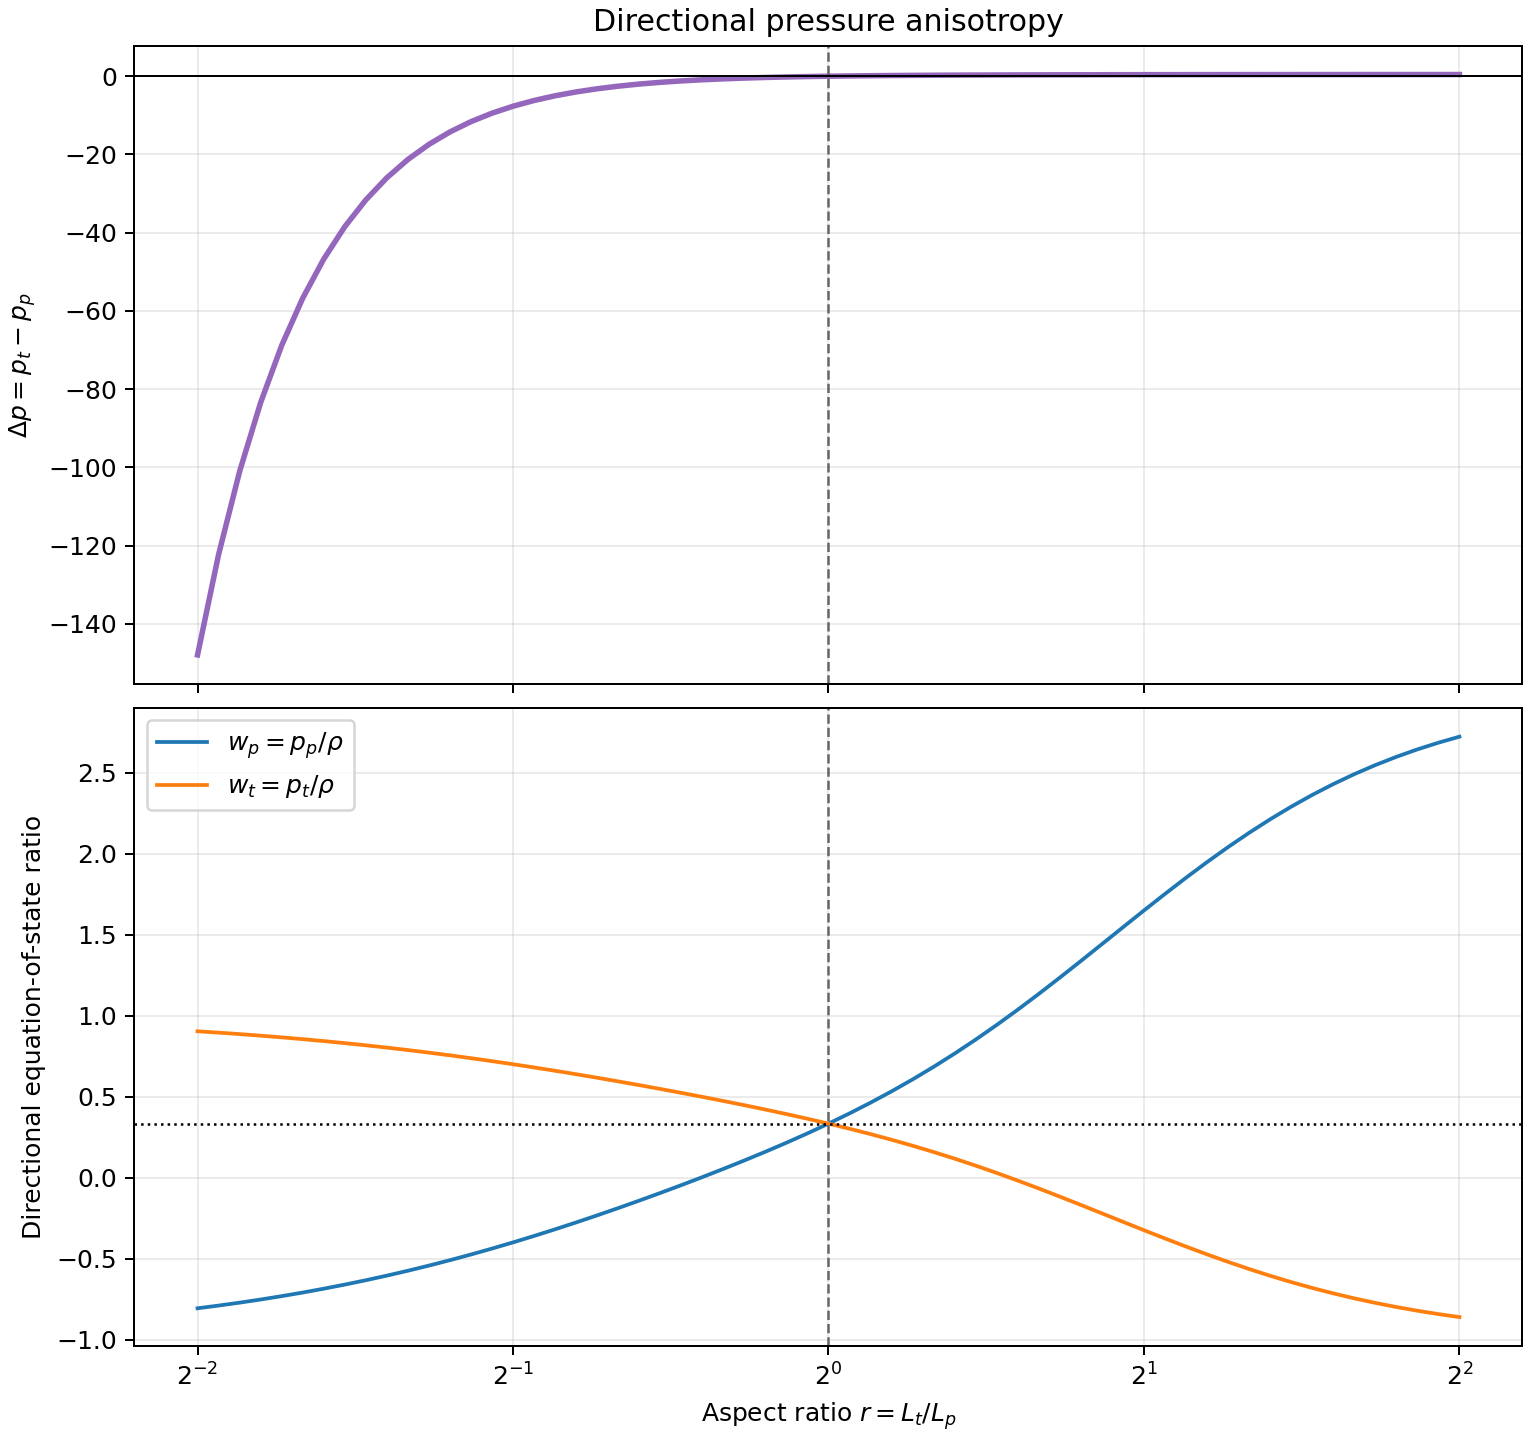
\includegraphics[width=\columnwidth]{cbr001_stage2_anisotropy.png}
\caption{Stage-2 biaxial anisotropy \(\Delta p=p_t-p_p\) versus shape ratio
\(r=L_t/L_p\).  The cubic point \(r=1\) is isotropic; anisotropy is shape
moduli dependent.}
\label{fig:stage2}
\end{figure}

% =============================================================================
\section{Biaxial free-field backreaction}
\label{sec:backreaction}

\subsection{Geometry and equations}

For the biaxial Bianchi-I line element
\begin{equation}
 \mathrm{d}s^2=-\mathrm{d}t^2+a_p^2\,\mathrm{d}x^2+a_t^2(\mathrm{d}y^2+\mathrm{d}z^2),
\end{equation}
define
\begin{equation}
 H=\frac{\Hp+2\Ht}{3},\qquad
 \delta=\Ht-\Hp,\qquad
 r=\frac{a_t}{a_p}.
\end{equation}
The shear system is the biaxial specialization of Bianchi-I
\cite{ellismaccallum1969}, with \(\kappa=8\pi G\),
\begin{equation}
 \dot\delta+3H\delta=\kappa(p_t-p_p),\qquad
 \dot r=r\delta,
 \label{eq:shear-system}
\end{equation}
and Hamiltonian constraint
\begin{equation}
 3H^2-\frac{\delta^2}{3}=\kappa\rho_{\mathrm{total}}.
 \label{eq:hamiltonian-biaxial}
\end{equation}
Stage~3A treats the verified Casimir tensor as a small radiation-like
perturbation (\(\propto a^{-4}\)) on a positive de~Sitter background and
integrates in \(N=\ln a\).
The dimensionless amplitude \(\epsilon\) absorbs \(\hbar c/L_\star^4\) relative
to the de~Sitter density scale (CBR-001 Stage~3A convention).
It validates the engine (perturbative limit, constraint and continuity
residuals) but does \emph{not} by itself establish any preferred Hubble ratio.

\subsection{The Stage-3B ratio test}

Let
\begin{equation}
 x=\frac{\delta}{H},\qquad
 q=\frac{\Ht}{\Hp}=\frac{1+x/3}{1-2x/3}.
 \label{eq:q-x}
\end{equation}
The historical target \(q=13/12\) corresponds to \(x_\star=3/38\).
The small-source fixed-background profile
\(x(N)=S(e^{-3N}-e^{-4N})\) peaks at \(N=\ln(4/3)\) with maximum
\((27/256)S\); merely reaching \(x_\star\) already requires
\(S\ge 128/171\simeq 0.7485\), outside the strict small-perturbation regime.

A nonlinear root search over initial shapes
\(r_0\in\{1.01,1.05,1.1,1.25,1.5,2,3,4\}\) and amplitudes spanning six decades
finds target-reaching thresholds for five of eight shapes.
Classification vocabulary:
\begin{itemize}
\item \texttt{NO\_CROSSING}: peak \(q\) stays below \(13/12\);
\item \texttt{TRANSIENT\_CROSSING}: touch or brief crossing;
\item \texttt{QUASI\_PLATEAU}: dwell \(\ge 1\) e-fold within \(1\%\) without
attractor criteria;
\item \texttt{ATTRACTOR}: dwell \(\ge 5\) e-folds within \(1\%\), nearby
trajectories converge, and no subsequent decay toward \(q=1\).
\end{itemize}
Results: zero attractors, zero quasi-plateaus, five transient crossings,
two no-crossings, one invalid (out-of-domain) shape
(Table~\ref{tab:stage3b}; Fig.~\ref{fig:ratio}).
Dwell times within \(1\%\) of the target are only
\(\sim 0.27\)--\(0.30\) e-folds.
Every valid candidate returns to \(q\to 1\) by \(N=20\), consistent with an
\(a^{-4}\) free-field source becoming negligible.
Nearby-trajectory stability tests confirm decay toward isotropy; none satisfy
attractor criteria.

\begin{table}[t]
\caption{Stage-3B classification at threshold amplitudes for the \(13/12\)
search.  ``Regime'' labels the peak Casimir energy fraction
(perturbative / marginal / nonperturbative).}
\label{tab:stage3b}
\begin{ruledtabular}
\begin{tabular}{lccc}
\(r_0\) & class & \(\epsilon_\star\) & regime \\
\hline
1.01 & no crossing & --- & --- \\
1.05 & no crossing & --- & --- \\
1.10 & transient & \(2.55\) & nonpert. \\
1.25 & transient & \(1.34\) & nonpert. \\
1.50 & transient & \(0.676\) & nonpert. \\
2.00 & transient & \(0.278\) & nonpert. \\
3.00 & transient & \(0.089\) & marginal \\
4.00 & invalid & --- & --- \\
\end{tabular}
\end{ruledtabular}
\end{table}

\begin{figure}[t]
\centering
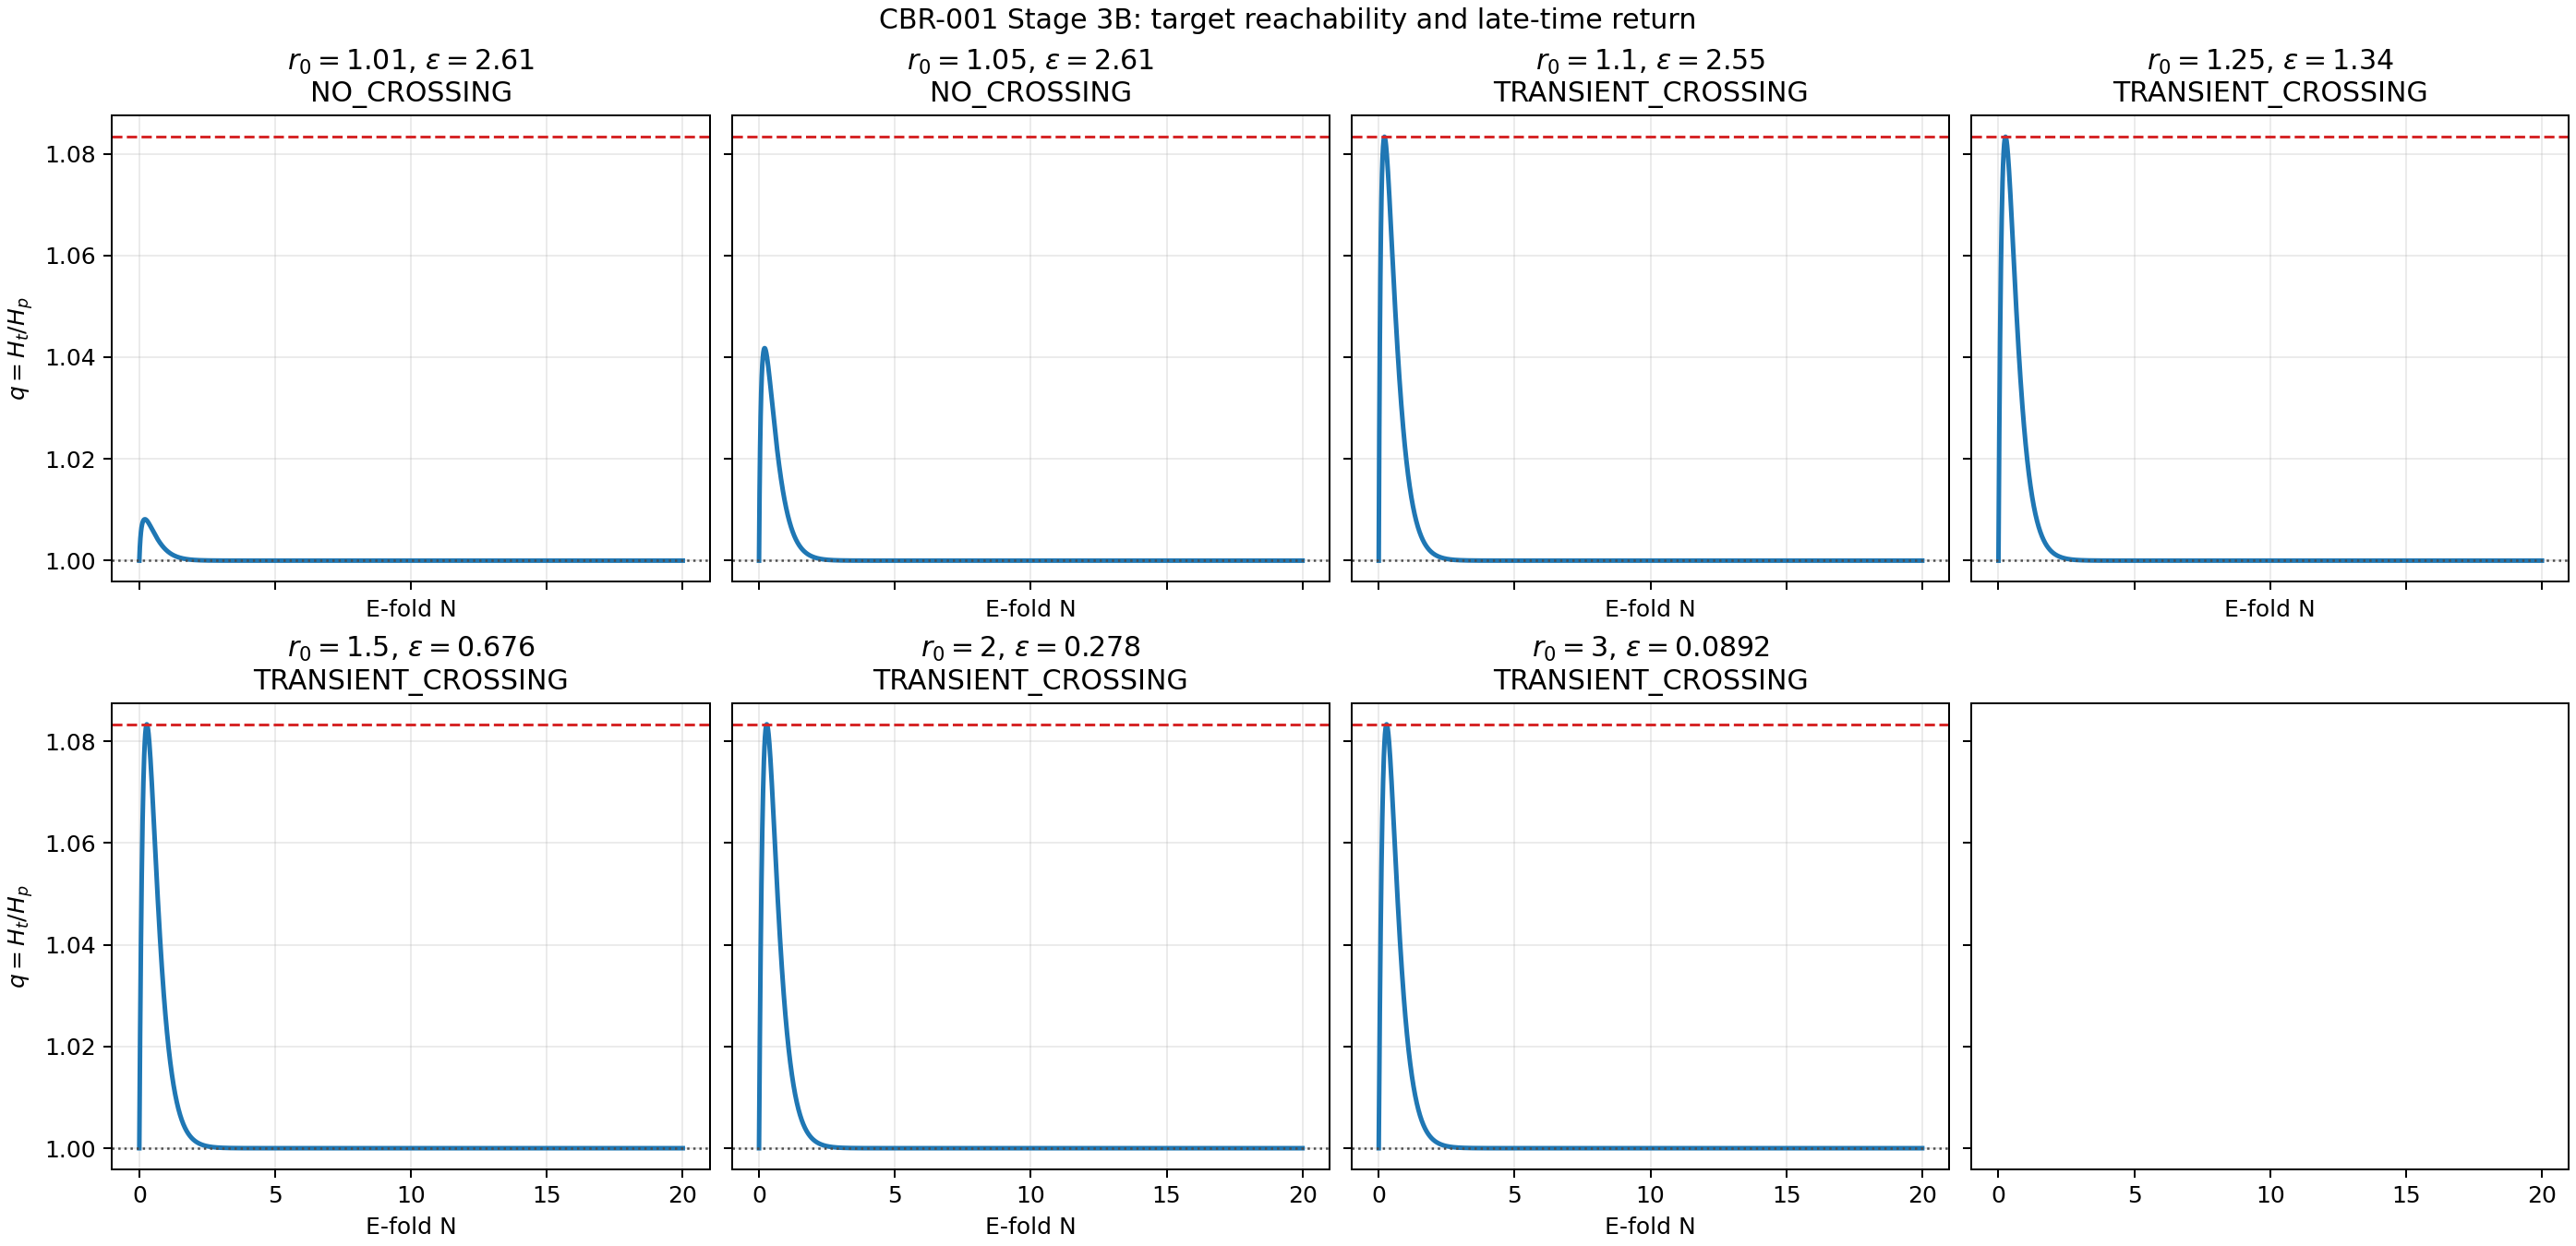
\includegraphics[width=\columnwidth]{cbr001_stage3b_ratio.png}
\caption{Representative Stage-3B trajectories of \(q=\Ht/\Hp\) versus \(N\).
The horizontal line marks \(13/12\).  Passages, when present, are brief;
late evolution returns to isotropy.}
\label{fig:ratio}
\end{figure}

\begin{figure}[t]
\centering
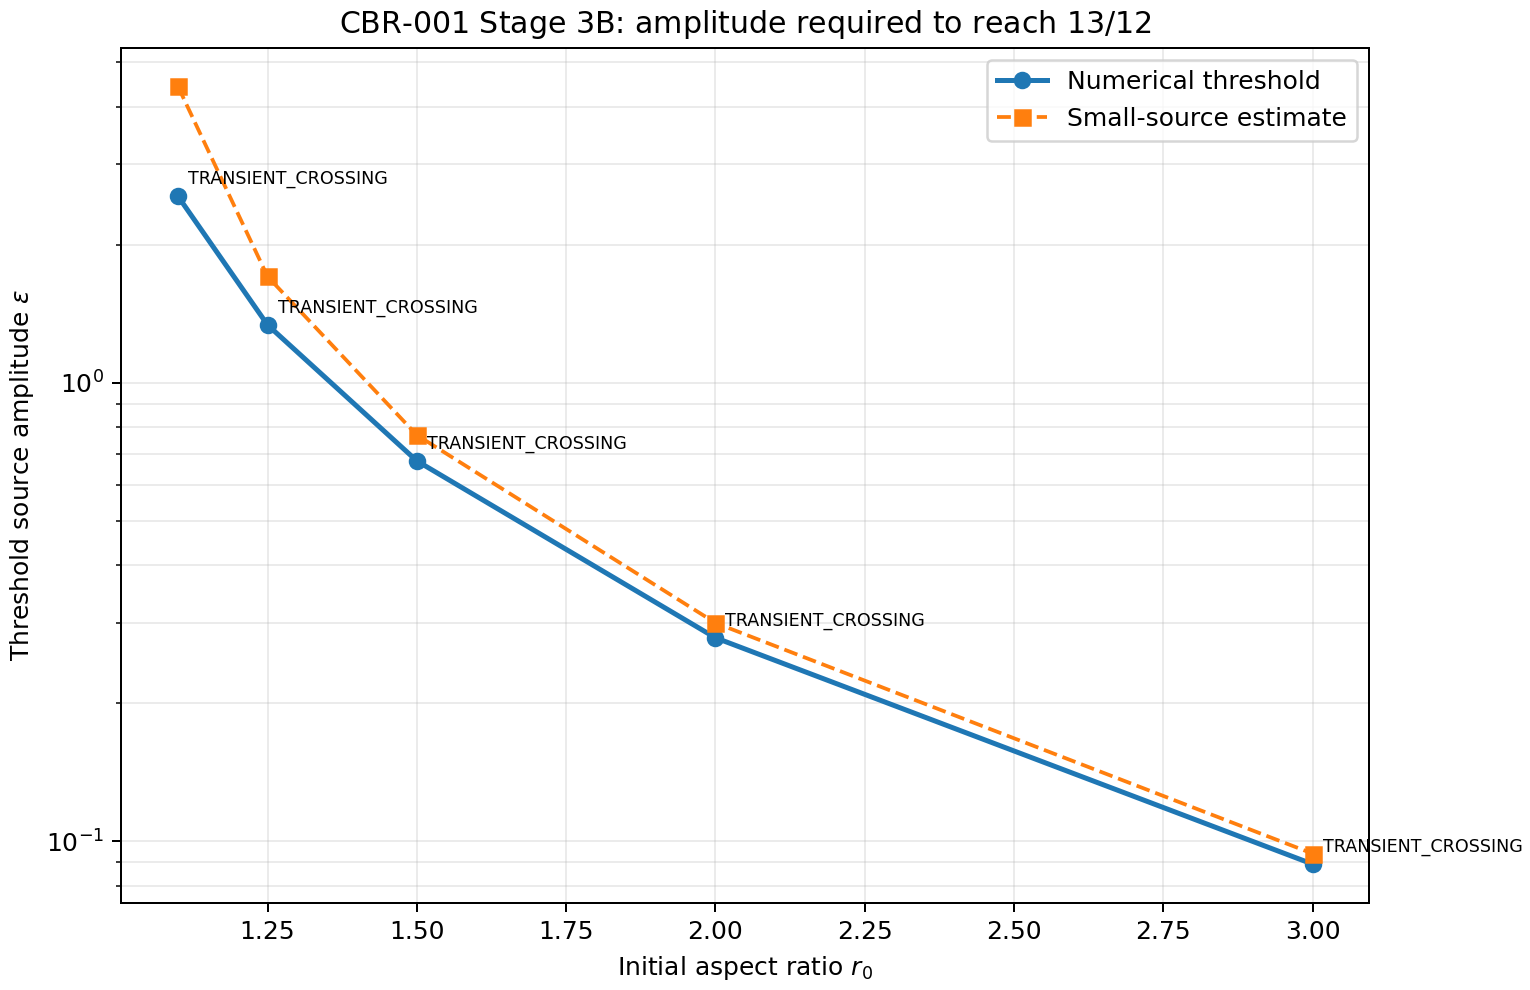
\includegraphics[width=\columnwidth]{cbr001_stage3b_threshold_epsilon.png}
\caption{Stage-3B threshold amplitudes \(\epsilon_\star(r_0)\) for first
touch of \(q=13/12\).  Near-cubic shapes require large free-field amplitudes;
no threshold defines an attractor.}
\label{fig:threshold}
\end{figure}

\subsection{Kinematic warning}

Because \(\mathrm{d}\ln r/\mathrm{d}N=x\), a constant \(q\neq 1\) requires
continuous evolution of the shape ratio; it is not a fixed-torus property.
A persistent anisotropic state would have to be a \emph{driven} solution with
an additional constitutive stress, not a free Casimir attractor.
For a prescribed \(x(N)\), the required anisotropic pressure is
\begin{equation}
 \Pi_{\mathrm{req}}=\frac{H^2}{\kappa}
 \Bigl[\frac{\mathrm{d}x}{\mathrm{d}N}
 +x\bigl(3+\tfrac{\mathrm{d}\ln H}{\mathrm{d}N}\bigr)\Bigr].
\end{equation}
In de~Sitter at fixed \(x=3/38\) this is \(\Pi_{\mathrm{req}}=9H^2/(38\kappa)\).
The free Casimir anisotropy scales as
\begin{equation}
 \Pi_{\mathrm{Cas}}\propto a^{-4}\,r^{8/3}
 \bigl[\widehat p_t(r)-\widehat p_p(r)\bigr]
\end{equation}
and cannot maintain \(\Pi_{\mathrm{req}}\) once the source redshifts away.
Any future positive claim of a persistent \(13/12\)-class ratio must derive
that extra stress (open programme CBR-002) without inserting the target into a
coefficient by hand.

% =============================================================================
\section{Historical packaging (explicitly not restored)}
\label{sec:history}

Cycle counting that assigns a fixed fraction \(1/12\) per compact direction and
promotes \(\Ht/\Hp=13/12\) to a free-field prediction, together with the
numerical map \(H_p=67.36\,\mathrm{km\,s^{-1}\,Mpc^{-1}}\Rightarrow
H_t=72.97\,\mathrm{km\,s^{-1}\,Mpc^{-1}}\), is a packaging of the \emph{question}
this paper tests---not a result we endorse.
The lattice stress is shape dependent; free-field backreaction does not lock
the ratio; and CMB topology bounds on cubic \(E_1\) cells
\cite{planck_topology,compact_promise} are a separate observational sector that
this rectangular free-field simulation does not claim to satisfy.

We likewise do not claim that rectangular Casimir stress derives a galactic
acceleration scale, fixes weak-field matching coefficients, or resolves the
Hubble tension \cite{planck,riess2022}.

% =============================================================================
\section{Limitations and open routes}
\label{sec:limits}

\begin{itemize}
\item Free massless scalar only; interacting or multi-field sectors untested.
\item Rectangular moduli; twisted flat spaces (\(E_2\), \(E_3\)) not scanned.
\item Positive de~Sitter testbed with Casimir as a small perturbation---not a
Casimir-dominated universe.
\item Persistent anisotropy requires a derived driven or memory stress
(CBR-002), not free-field packaging.
\item CMB compatibility of any particular \((L_i)\) is not established here.
\end{itemize}

These limitations are research boundaries, not research bans: driven
constitutive stress, alternate topologies, and richer field content remain
open under an honest claim ladder.

% =============================================================================
\section{Conclusions}
\label{sec:concl}

A free massless scalar on rectangular flat \(\Tthree\) yields a validated,
shape-dependent anisotropic Casimir stress.
When that stress backreacts as a small \(a^{-4}\) source on biaxial de~Sitter
expansion, the ratio \(\Ht/\Hp=13/12\) appears at most as a brief transient at
large free-field amplitudes, never as a quasi-plateau or attractor in the
search reported here.
Free Casimir stress alone therefore cannot sustain the historically proposed
anisotropic expansion, nor justify a free-field map to
\(H_t=72.97\,\mathrm{km\,s^{-1}\,Mpc^{-1}}\).
Public code and stage summaries under \texttt{Analysis/Casimir/CBR-001/}
reproduce the Stage-1--3B pipeline.
Frozen SHA-256 anchors for the numerical tables used here are recorded in the
paper repository file \texttt{CBR001\_CHECKSUMS.md} (data and code availability
for this draft).

\begin{acknowledgments}
Computations use the repository environment \texttt{itsm\_env} and the
CBR-001 gate package.
Claim hygiene for related geometric packaging is recorded in companion note
\cite{boyd_p1}.
\end{acknowledgments}

\appendix

\section{Reproducibility anchors}
\label{app:checksums}

Table~\ref{tab:checksums} lists SHA-256 digests of the CBR-001 CSV/JSON
artifacts underlying the Stage-1--3B numbers in the main text (branch
\texttt{recovery/v12-core-architecture}, freeze date 2026-08-01).
Re-running the Stage scripts after intentional code changes will alter digests;
any published revision must update this table.

\begin{table}[h]
\caption{SHA-256 of CBR-001 artifacts used in this draft.}
\label{tab:checksums}
\begin{ruledtabular}
\begin{tabular}{ll}
Artifact & SHA-256 (prefix) \\
\hline
\texttt{cbr001\_stage1.csv} & \texttt{9E6874226FAA\ldots} \\
\texttt{cbr001\_stage2\_scan.csv} & \texttt{9257F3A67CB5\ldots} \\
\texttt{cbr001\_stage3b\_thresholds.csv} & \texttt{370B02480FF0\ldots} \\
\texttt{cbr001\_stage3b\_summary.json} & \texttt{4AD9223CE32C\ldots} \\
\end{tabular}
\end{ruledtabular}
\end{table}

Full digests and reproduction commands appear in
\texttt{papers/P2-Rectangular-T3-Casimir/CBR001\_CHECKSUMS.md}.

\bibliography{references}

\end{document}
